% !TeX program = xelatex
% Build from the repository root: latexmk -xelatex -cd Presentation/presentation.tex
\RequirePackage{fix-cm}
\documentclass[10pt,aspectratio=169]{beamer}
% A 16:9 canvas sized for readable 24-point-equivalent body text on screen.
\geometry{paperwidth=192mm,paperheight=108mm}

% The repository's original Metropolis template, adapted for this presentation.
\usetheme[progressbar=frametitle,sectionpage=none,numbering=fraction]{metropolis}
\usepackage{appendixnumberbeamer}
\usepackage{booktabs}
\usepackage{tabularx}
\usepackage{array}
\usepackage{graphicx}
\usepackage{tikz}
\usepackage{pgfplots}
\usepackage{bibentry}
\usetikzlibrary{arrows.meta,positioning,calc}
\AtBeginDocument{\pgfplotsset{compat=1.18}}
\graphicspath{{figures/}}

\setsansfont{FiraSans}[
  Extension=.otf,UprightFont=*-Regular,ItalicFont=*-Italic,
  BoldFont=*-SemiBold,BoldItalicFont=*-SemiBoldItalic
]

\definecolor{HSGGreen}{HTML}{00843D}
\definecolor{Ink}{HTML}{17352D}
\definecolor{Muted}{HTML}{60716B}
\definecolor{Mist}{HTML}{F0F5F2}
\definecolor{Rule}{HTML}{D7E3DC}
\definecolor{ChartBlue}{HTML}{4682B4}
\definecolor{ChartCoral}{HTML}{D96C4A}

\setbeamercolor{normal text}{fg=Ink,bg=white}
\setbeamercolor{frametitle}{fg=Ink,bg=white}
\setbeamercolor{alerted text}{fg=HSGGreen}
\setbeamercolor{progress bar}{fg=HSGGreen,bg=Rule}
\setbeamercolor{title separator}{fg=HSGGreen}
\setbeamercolor{palette primary}{fg=white,bg=Ink}
\setbeamercolor{block title}{fg=HSGGreen,bg=Mist}
\setbeamercolor{block body}{fg=Ink,bg=Mist}
\setbeamercolor{takeaway}{fg=Ink,bg=Mist}
\setbeamercolor{page number in head/foot}{fg=Muted}
\setbeamerfont{frametitle}{size=\large,series=\bfseries}
\setbeamerfont{footline}{size=\fontsize{6.5}{8}\selectfont}
\setbeamerfont{page number in head/foot}{size=\fontsize{6.5}{8}\selectfont}
\setbeamersize{text margin left=9mm,text margin right=9mm}
\setbeamertemplate{navigation symbols}{}
\setbeamertemplate{frame footer}{Machine Learning in Finance\enspace /\enspace\insertsectionhead}
\setlength{\tabcolsep}{5pt}
\setlength{\parskip}{0pt}
\renewcommand{\arraystretch}{1.18}
\hypersetup{
  pdftitle={Reading IMF Programs on Day One},
  pdfauthor={Mathis Clément; Ethan Moore; Ali Haidar; Tristan Zemp; Joao Matteo Pisaturo; José Pablo Caldas},
  pdfsubject={Approval-time prediction of IMF programme interruptions},
  colorlinks=true,linkcolor=HSGGreen,citecolor=Muted,urlcolor=HSGGreen
}
\pdfstringdefDisableCommands{\def\translate#1{#1}}

\newcommand{\eyebrow}[1]{%
  \par\noindent{\color{HSGGreen}\scriptsize\bfseries\MakeUppercase{#1}\par}\vspace{1mm}}
\newcommand{\source}[1]{%
  \par\vspace{1.5mm}{\fontsize{6.5}{8}\selectfont\color{Muted}#1\par}}
\newcommand{\takeaway}[1]{%
  \par\vspace{2mm}\begin{beamercolorbox}[wd=\linewidth,sep=2mm]{takeaway}%
    \small\bfseries #1
  \end{beamercolorbox}}
\newcommand{\point}[2]{%
  \par\noindent\textbf{#1}\par{\small #2\par}\vspace{2.5mm}}
\newcommand{\metric}[3]{%
  \par\noindent{\fontsize{25}{28}\selectfont\bfseries\color{HSGGreen}#1\par}%
  \vspace{0.5mm}{\small\bfseries #2\par}%
  {\scriptsize\color{Muted}#3\par}}
\newcommand{\refentry}[1]{%
  {\let\newblock\space\bibentry{#1}.\par}\vspace{3mm}}

\title{Reading IMF Programs on Day One}
\subtitle{Machine learning on 173 IMF lending programmes, 2002--2016}
\author{Mathis Clément \and Ethan Moore \and Ali Haidar \and Tristan Zemp
  \and Joao Matteo Pisaturo \and José Pablo Caldas}
\institute{University of St. Gallen}
\date{7 October 2026}

\begin{document}
\bibliographystyle{apalike}

% 1. Title --------------------------------------------------------------------
{\setbeamertemplate{footline}{}
\begin{frame}[plain,noframenumbering]
  \nobibliography{references}
  \begin{tikzpicture}[remember picture,overlay]
    \fill[Mist] ([xshift=-44mm]current page.north east)
      rectangle (current page.south east);
    \fill[HSGGreen] (current page.north west)
      rectangle ([xshift=2mm]current page.south west);
    \node[anchor=north west,inner sep=0] at
      ([xshift=11mm,yshift=-9mm]current page.north west)
      {
\includegraphics[width=45mm]{hsg_logo.png}};
    \node[anchor=north west,inner sep=0,text width=130mm] at
      ([xshift=11mm,yshift=-30mm]current page.north west) {
      {\fontsize{30}{35}\selectfont\bfseries Reading IMF Programs\\on Day One\par}
      \vspace{4mm}
      {\fontsize{12}{16}\selectfont Machine learning on 173 IMF lending programmes\\2002--2016\par}
    };
    \node[anchor=north west,inner sep=0,text width=130mm] at
      ([xshift=11mm,yshift=-81mm]current page.north west) {
      {\fontsize{9}{12}\selectfont
      \begin{tabular}{@{}lll@{}}
        Mathis Clément & Ethan Moore & Ali Haidar\\
        Tristan Zemp & Joao Matteo Pisaturo & José Pablo Caldas
      \end{tabular}\par}
      \vspace{4mm}
      {\fontsize{9}{11}\selectfont\color{Muted}University of St. Gallen\enspace\textbullet\enspace 7 October 2026}
    };
    \node[anchor=north west,inner sep=0,text width=34mm] at
      ([xshift=-37mm,yshift=-21mm]current page.north east) {
      \metric{173}{Programmes}{2002--2016}
      \vspace{8mm}
      \metric{13}{Predictors}{Known at approval}
      \vspace{8mm}
      \metric{3}{Models}{One prediction task}
    };
  \end{tikzpicture}
\end{frame}
}

% 2. Executive summary --------------------------------------------------------
\section{Overview}
\begin{frame}[t]{Executive summary}
  \vspace{1mm}
  \begin{columns}[T,onlytextwidth]
    \begin{column}{0.60\textwidth}
      \eyebrow{The question}
      {\large Can information available at approval predict permanent interruption?\par}
      \vspace{3mm}
      \point{A modest signal in development}{The random forest reaches about 0.63 balanced accuracy out of fold.}
      \point{No reliable test-set advantage}{With only 28 later programmes, performance is unstable and close to chance.}
      \point{Programme design is most informative}{Scheduled reviews, facility type and loan access lead the forest's importance ranking.}
    \end{column}
    \begin{column}{0.34\textwidth}
      \eyebrow{Road map}
      \small
      \begin{enumerate}
        \setlength{\itemsep}{2mm}
        \item Literature and research question
        \item Study goal
        \item Data and feature engineering
        \item Three prediction models
        \item Model comparison
        \item Limitations and conclusion
        \item Sources
      \end{enumerate}
    \end{column}
  \end{columns}
  \takeaway{Approval-day information contains some signal, but reliable out-of-sample prediction remains difficult.}
\end{frame}

% 3. Literature ---------------------------------------------------------------
\section{Research question}
\begin{frame}[t]{Why predict interruption at approval?}
  \vspace{1mm}
  \begin{columns}[T,onlytextwidth]
    \begin{column}{0.51\textwidth}
      \small
      \point{Financial relevance}{Interruptions can weaken investor confidence and sovereign financing credibility.}
      \point{Politics and conditionality}{Political incentives and institutional capacity affect implementation; evidence on structural conditions is mixed.}
      {\scriptsize\color{Muted}Ivanova et al. (2003); Joyce (2006); Reinsberg et al. (2022).\par}
      \vspace{2mm}
      \point{The gap in machine learning}{Existing studies predict IMF participation. We ask whether approval-time information predicts permanent interruption.}
      {\scriptsize\color{Muted}Agbloyor et al. (2023); Batsuuri et al. (2024).\par}
    \end{column}
    \begin{column}{0.44\textwidth}
      \eyebrow{Timing of IMF programme disbursements}
      \vspace{3mm}
      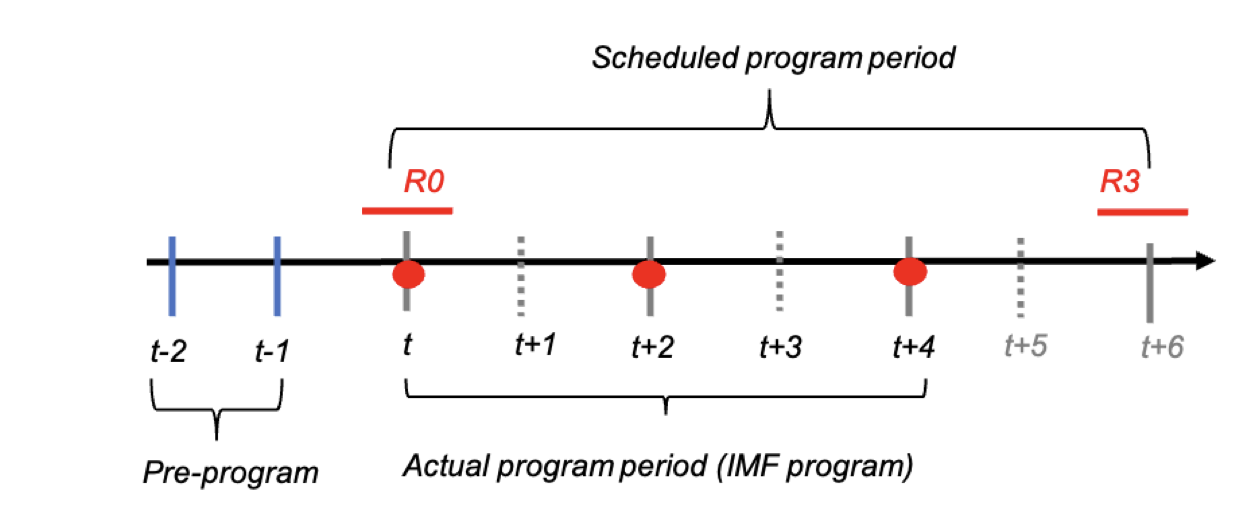
\includegraphics[width=\linewidth]{disbursement_timeline.png}
      \source{Source: Aiyar and Patnam (2021), IMF Working Paper 21/146, Figure 2, p.\ 8.}
      \vspace{3mm}
      \small A programme can end before its scheduled final review. The prediction must be made at \alert{Board approval}.
    \end{column}
  \end{columns}
  \takeaway{Can information available at approval predict permanent interruption?}
\end{frame}

% 4. Goal and selection -------------------------------------------------------
\section{Study design}
\begin{frame}[t]{Study goal and sample}
  \vspace{1mm}
  \begin{columns}[T,onlytextwidth]
    \begin{column}{0.48\textwidth}
      \eyebrow{Binary classification}
      \small
      \textbf{Outcome: programme interruption}
      \[
        Y=\begin{cases}
          1 & \text{at least one scheduled review}\\[-1mm]
            & \text{was never completed},\\[1mm]
          0 & \text{otherwise.}
        \end{cases}
      \]
      \[\Pr(Y=1\mid X)=f(X),\qquad X=(X_1,\ldots,X_{13}).\]
      \vspace{1mm}
      Deal design, conditions, track record and macroeconomic information observed at approval.
      \takeaway{Purpose: prediction, not causal explanation.}
      \source{Predictive framing: Shmueli (2010); James et al. (2013).}
    \end{column}
    \begin{column}{0.46\textwidth}
      \eyebrow{Which programmes enter the sample?}
      \small
      \begin{enumerate}
        \setlength{\itemsep}{2mm}
        \item \textbf{Review-based facilities:} SBA, EFF, ECF and SCF, including predecessors.
        \item \textbf{Approval in 2002--2016:} MONA review records start in 2002.
        \item \textbf{Money at stake:} non-precautionary arrangements with positive drawings.
        \item \textbf{Observed outcome:} matched review records.
        \item \textbf{Blends merged:} same country and approval date count as one programme.
      \end{enumerate}
      \source{Earlier risk flags could help calibrate conditionality and inform sovereign-risk pricing.}
    \end{column}
  \end{columns}
\end{frame}

% 5. Data sources -------------------------------------------------------------
\section{Data and features}
\begin{frame}[t]{From raw records to programme-level data}
  \vspace{1mm}
  \begin{columns}[T,onlytextwidth]
    \begin{column}{0.60\textwidth}
      \eyebrow{Data sources and their roles}
      \fontsize{8.5}{11}\selectfont
      \begin{tabularx}{\linewidth}{@{}>{\raggedright\arraybackslash\bfseries}p{2.55cm}>{\raggedright\arraybackslash}X@{}}
        \toprule
        Source & Information collected \\
        \midrule
        IMF commitments & Dates, approved and drawn amounts, access as a share of quota, facility type.\\
        MONA reviews & Scheduled and completed reviews; construction of the outcome.\\
        MONA conditions and purchases & Structural conditions, prior actions and candidate front-loading measures.\\
        MONA economic indicators & Approval-snapshot growth, inflation and current account.\\
        WEO / WDI & WEO (Apr.\ 2026): debt and net lending. WDI: growth / inflation fallback considered. Final macro inputs use MONA.\\
        \bottomrule
      \end{tabularx}
      \source{IMF (2026a--c); World Bank (2026). Revised WEO fiscal data are excluded from the prediction inputs.}
    \end{column}
    \begin{column}{0.35\textwidth}
      \eyebrow{Construction pipeline}
      \metric{1,576}{Raw arrangements}{Five raw files; no shared identifier}
      \vspace{3mm}
      \small
      \textbf{Link} by country and closest approval date within $\pm60$ days.\par
      \vspace{2mm}
      \textbf{Merge} blends and compare reviews scheduled at approval with those completed.\par
      \vspace{3mm}
      \metric{173}{Programme observations}{82 interrupted / 91 completed}
    \end{column}
  \end{columns}
\end{frame}

% 6. Feature engineering ------------------------------------------------------
\begin{frame}[t]{Thirteen inputs, all known at approval}
  \vspace{1mm}
  \begin{columns}[T,onlytextwidth]
    \begin{column}{0.48\textwidth}
      \eyebrow{01 / Deal design · 5 inputs}
      \small
      Log access (\% of quota); planned duration; scheduled reviews; concessional facility; extended facility.\par
      \vspace{5mm}
      \eyebrow{02 / Conditionality · 2 inputs}
      Structural conditions and prior actions at approval.
    \end{column}
    \begin{column}{0.47\textwidth}
      \eyebrow{03 / Track record · 3 inputs}
      \small
      Prior programmes over 20 years; time since the previous programme; no previous track record.\par
      \vspace{5mm}
      \eyebrow{04 / Macroeconomy · 3 inputs}
      Real GDP growth; CPI inflation; current account as a share of GDP, from the approval snapshot.
    \end{column}
  \end{columns}
  \vspace{5mm}
  \begin{beamercolorbox}[wd=\linewidth,sep=2.5mm]{takeaway}
    \eyebrow{Twelve candidate entries excluded}
    \small
    \begin{tabularx}{\dimexpr\linewidth-5mm\relax}{@{}*{4}{>{\raggedright\arraybackslash}X}@{}}
      \textbf{6 look-ahead} & \textbf{4 redundant / fragile} & \textbf{1 missing-data} & \textbf{1 identifier group}\\
      Post-approval outcomes and revised data & Duplicate design or history measures & Fiscal indicators with too many gaps & Country and approval dates
    \end{tabularx}
  \end{beamercolorbox}
  \source{Output: \texttt{interrupted} (0/1). Feature definitions and exclusion audit: \texttt{Data\_Prep/01\_data.R}.}
\end{frame}

% 7. Descriptive evidence -----------------------------------------------------
\begin{frame}[t]{Exploration: programme design stands out}
  \vspace{1mm}
  \begin{columns}[T,onlytextwidth]
    \begin{column}{0.47\textwidth}
      \eyebrow{Interruption rate by facility}
      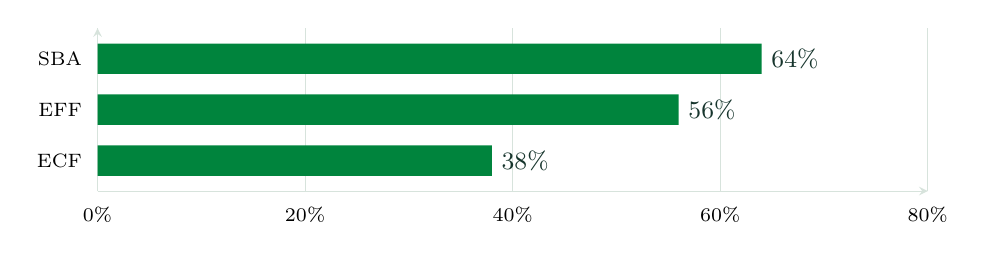
\begin{tikzpicture}
        \begin{axis}[
          width=\linewidth,height=3.65cm,
          xbar,bar width=11pt,xmin=0,xmax=80,
          symbolic y coords={ECF,EFF,SBA},ytick=data,
          xtick={0,20,40,60,80},xticklabel={\pgfmathprintnumber{\tick}\%},
          axis lines=left,axis line style={Rule},tick style={draw=none},
          xmajorgrids=true,grid style={Rule},
          tick label style={font=\scriptsize},
          nodes near coords={\pgfmathprintnumber\pgfplotspointmeta\%},
          every node near coord/.append style={font=\small,color=Ink},
          enlarge y limits=0.3,
        ]
          \addplot[fill=HSGGreen,draw=none] coordinates {(38,ECF) (56,EFF) (64,SBA)};
        \end{axis}
      \end{tikzpicture}
      \source{Selected facilities; rounded rates reported in the original presentation.}
      \vspace{1mm}
      \small Interruption rises from \textbf{38\% in 2002--07} to \textbf{61\% in 2014--16}.
    \end{column}
    \begin{column}{0.48\textwidth}
      \point{More reviews, larger programmes}{Interrupted programmes have 7.3 scheduled reviews versus 5.9; access is larger and concessional / extended facilities are less common ($p\leq0.004$).}
      \point{Weak individual correlations}{Reviews: 0.31; access: 0.25; concessional: $-0.22$. Conditions, macro and track record show no clear outcome differences.}
      \point{Overlap and non-linearity}{Concessional--extended correlation: 0.72. Interruption across access quartiles: 31 / 52 / 41 / 67\%.}
      \small These patterns motivate testing flexible models alongside a linear log-odds benchmark.
    \end{column}
  \end{columns}
  \source{Descriptive evidence: full sample, n = 173; these associations are not causal effects.}
\end{frame}

% 8. Forest tuning ------------------------------------------------------------
\section{Random forest}
\begin{frame}[t]{Random forest: tuning is relatively flat}
  \vspace{1mm}
  \small
  \textbf{24 settings:} 6 \texttt{mtry} values $\times$ 4 tree counts; balanced accuracy under three validation schemes.
  \vspace{1mm}
  \begin{center}
    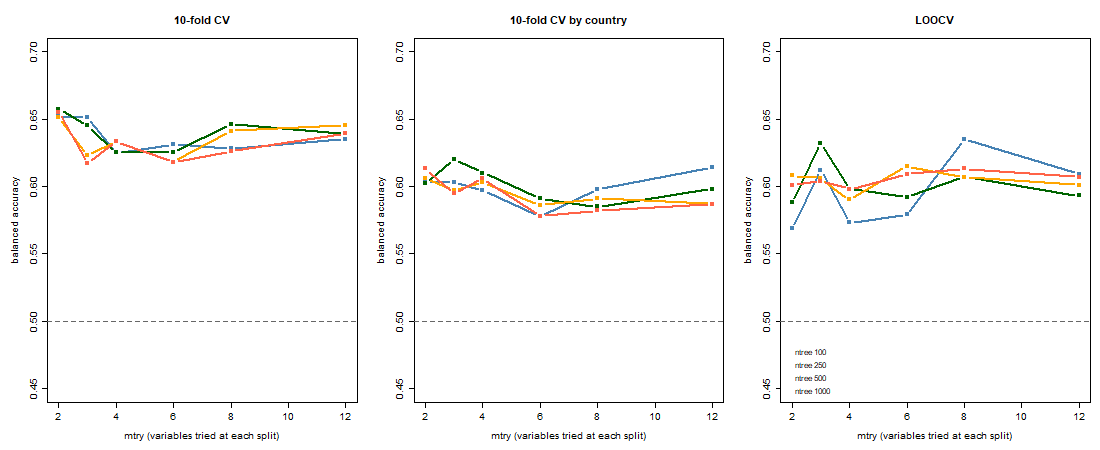
\includegraphics[width=0.97\linewidth,height=6.05cm,keepaspectratio]{rf_tuning.png}
  \end{center}
  \vspace{-2mm}
  \begin{columns}[T,onlytextwidth]
    \begin{column}{0.48\textwidth}
      \small \textbf{Flat grid.} Curves cross and scores stay within roughly five percentage points; no setting dominates.
    \end{column}
    \begin{column}{0.48\textwidth}
      \small \textbf{Selected with country CV:} 250 trees, \texttt{mtry} = 3; balanced accuracy \alert{0.620}.
    \end{column}
  \end{columns}
  \source{Country-grouped validation holds out entire countries, giving the most conservative tuning scores here. Source: original random-forest tuning figure.}
\end{frame}

% 9. Forest results -----------------------------------------------------------
\begin{frame}[t]{Random forest: the test signal is weak}
  \vspace{1mm}
  \begin{columns}[T,onlytextwidth]
    \begin{column}{0.55\textwidth}
      \eyebrow{Development and test performance}
      \small
      \begin{tabularx}{\linewidth}{@{}Xrr@{}}
        \toprule
        & Accuracy & Balanced acc.\\
        \midrule
        Development, out of fold & 0.641 & \textbf{0.630}\\
        Test, final forest & 0.500 & \textbf{0.508}\\
        Test, always interrupted & 0.607 & 0.500\\
        \bottomrule
      \end{tabularx}\par
      \vspace{4mm}
      \point{Correctly identified on the test set}{8 of 17 interrupted programmes; 6 of 11 completed programmes.}
      \small Development scores use out-of-fold predictions; final performance is measured on later programmes.
    \end{column}
    \begin{column}{0.39\textwidth}
      \eyebrow{Substantial uncertainty}
      \metric{0.51--0.64}{Balanced accuracy}{Across 20 random seeds}
      \vspace{5mm}
      \metric{0.38--0.75}{Bootstrap interval}{Reported 95\% interval; includes 0.50}
      \vspace{3mm}
      \small With only 28 test observations, the result is sensitive to random variation.
    \end{column}
  \end{columns}
  \takeaway{The development signal does not translate into a reliable test-set edge over chance.}
\end{frame}

% 10. Forest importance -------------------------------------------------------
\begin{frame}[t]{Random forest: programme design leads}
  \vspace{1mm}
  \begin{columns}[T,onlytextwidth]
    \begin{column}{0.60\textwidth}
      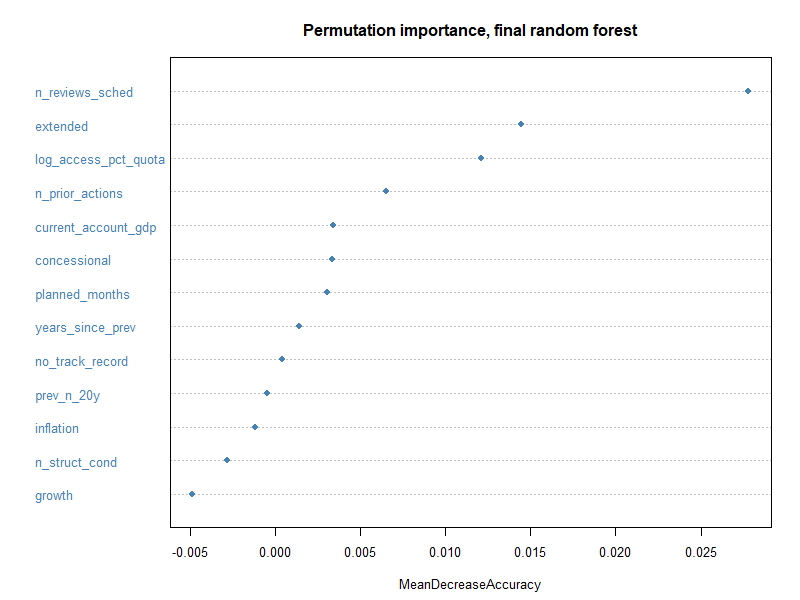
\includegraphics[width=\linewidth,height=6.8cm,keepaspectratio]{rf_importance.png}
      \source{Permutation importance: mean decrease in accuracy after shuffling each predictor.}
    \end{column}
    \begin{column}{0.35\textwidth}
      \eyebrow{The strongest predictors}
      \small
      \begin{enumerate}
        \setlength{\itemsep}{3mm}
        \item Number of scheduled reviews
        \item Extended facility indicator
        \item Loan access (\% of quota, log)
      \end{enumerate}
      \vspace{3mm}
      Macro variables have little importance here; growth and inflation are at or below zero.
      \takeaway{Predictive importance is not a causal effect.}
    \end{column}
  \end{columns}
\end{frame}

% 11. Logistic regression -----------------------------------------------------
\section{Logistic regression}
\begin{frame}[t]{Logistic regression: a transparent benchmark}
  \vspace{1mm}
  \begin{columns}[T,onlytextwidth]
    \begin{column}{0.47\textwidth}
      \eyebrow{Test-set performance}
      \scriptsize
      \begin{tabularx}{\linewidth}{@{}Xrr@{}}
        \toprule
        & Logistic & Forest\\
        \midrule
        Accuracy & 0.536 & 0.500\\
        Balanced accuracy & 0.570 & 0.508\\
        AUC & \textbf{0.684} & 0.586\\
        \bottomrule
      \end{tabularx}
      \vspace{1mm}
      \begin{center}
        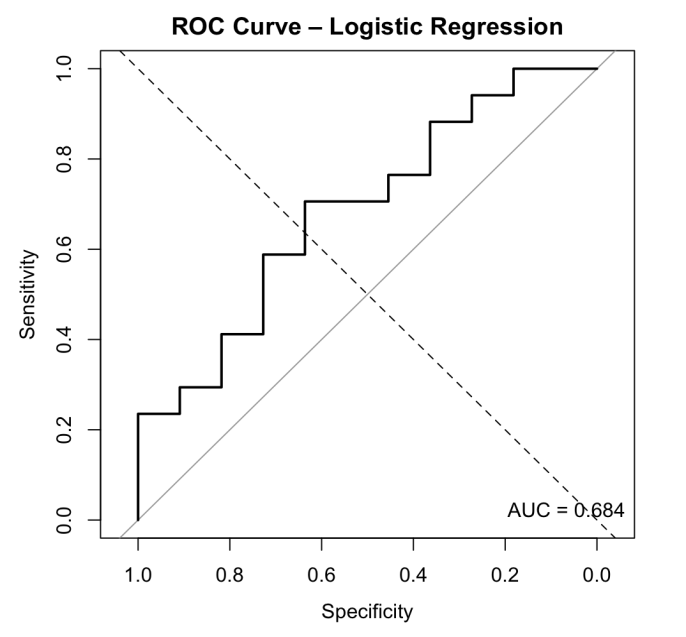
\includegraphics[height=4.4cm,width=\linewidth,keepaspectratio]{logit_roc.png}
      \end{center}
    \end{column}
    \begin{column}{0.48\textwidth}
      \eyebrow{Interpretability}
      \begin{center}
        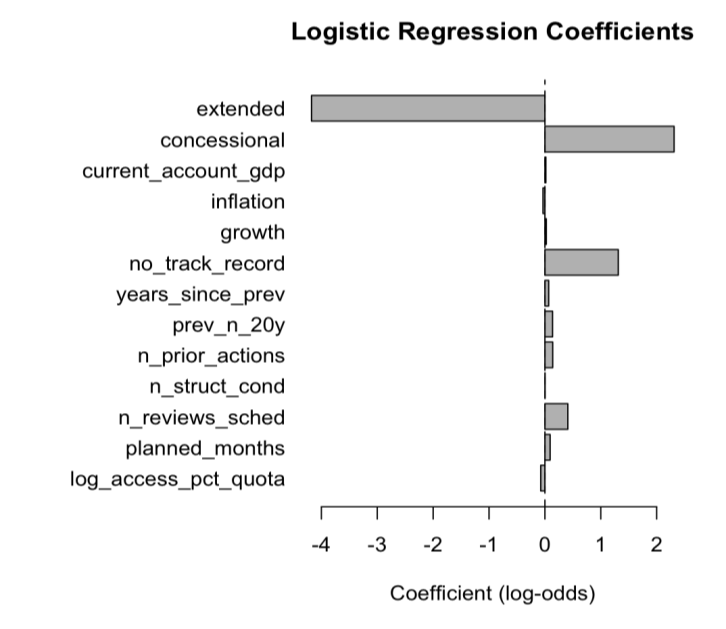
\includegraphics[height=4.95cm,width=\linewidth,keepaspectratio]{logit_coefficients.png}
      \end{center}
      \vspace{-2mm}
      \small
      \textbf{Logistic:} Interpretable coefficient direction \& magnitude; less flexible.\par
      \vspace{1mm}
      \textbf{Forest:} captures non-linearities; more flexible, harder to interpret.
    \end{column}
  \end{columns}
  \source{Coefficient magnitudes depend on the units of each predictor; they are not directly comparable measures of importance.}
\end{frame}

% 12. Neural network ----------------------------------------------------------
\section{Neural network}
\begin{frame}[t]{Neural network: small is enough}
  \vspace{1mm}
  \begin{columns}[T,onlytextwidth]
    \begin{column}{0.60\textwidth}
      \eyebrow{Country-grouped 10-fold cross-validation}
      \vspace{3mm}
      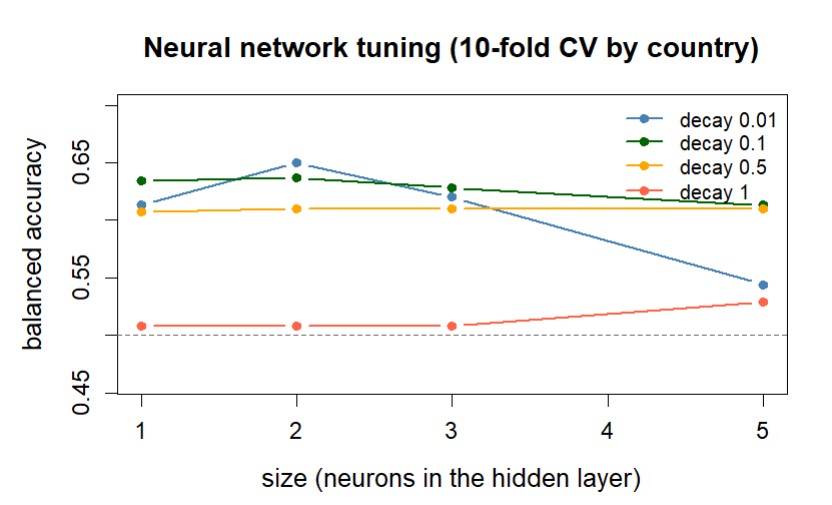
\includegraphics[width=\linewidth,height=5.8cm,keepaspectratio]{nn_tuning.png}
      \source{One hidden layer. Size: 1, 2, 3 or 5 neurons; weight decay: 0.01, 0.1, 0.5 or 1.}
    \end{column}
    \begin{column}{0.35\textwidth}
      \point{A compact network performs best}{Two neurons and a light penalty (decay 0.01) give the highest tuning score, about 0.65.}
      \point{More capacity can hurt}{With light regularisation, increasing from two to five neurons reduces the score to about 0.54.}
      \point{Heavy regularisation underfits}{With decay 1, performance stays near chance (roughly 0.51--0.53).}
    \end{column}
  \end{columns}
  \takeaway{With 145 training programmes, added model complexity does not guarantee better predictions.}
\end{frame}

% 13. Comparison --------------------------------------------------------------
\section{Model comparison}
\begin{frame}[t]{Model comparison: no reliable winner}
  \vspace{1mm}
  \begin{columns}[T,onlytextwidth]
    \begin{column}{0.56\textwidth}
      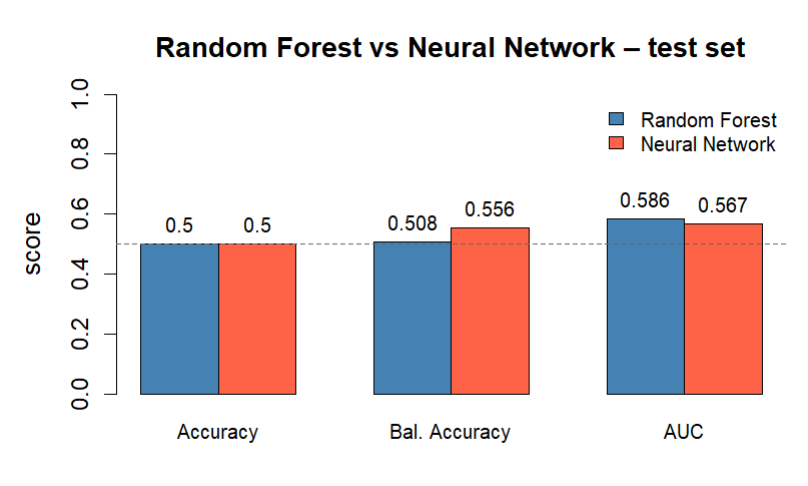
\includegraphics[width=\linewidth]{model_comparison.png}
      \source{Original test-set comparison. The 0.50 line is a chance reference for balanced accuracy and AUC, not the majority-class accuracy benchmark.}
    \end{column}
    \begin{column}{0.40\textwidth}
      \eyebrow{All models / same 28 test programmes}
      \fontsize{8}{10}\selectfont
      \begin{tabularx}{\linewidth}{@{}Xrrr@{}}
        \toprule
        Model & Acc. & BA & AUC\\
        \midrule
        Logistic & 0.536 & 0.570 & 0.684\\
        Forest & 0.500 & 0.508 & 0.586\\
        Neural net & 0.500 & 0.556 & 0.567\\
        \midrule
        Always 1 & 0.607 & 0.500 & 0.500\\
        \bottomrule
      \end{tabularx}\par
      \vspace{4mm}
      \small
      Neither the forest nor the neural network is reliably better than the other.\par
      \vspace{3mm}
      Logistic regression has the highest reported BA and AUC, but this small test sample cannot establish a reliable ranking.
    \end{column}
  \end{columns}
  \takeaway{More flexible models do not demonstrate a dependable advantage in this sample.}
\end{frame}

% 14. Conclusion --------------------------------------------------------------
\section{Conclusion}
\begin{frame}[t]{Limitations and conclusion}
  \vspace{1mm}
  \begin{columns}[T,onlytextwidth]
    \begin{column}{0.47\textwidth}
      \eyebrow{What limits the evidence}
      \point{Small sample}{145 training and 28 test programmes, with only 11 completed. One extra correct prediction changes BA by about 0.03--0.05.}
      \point{One time split}{The interruption share rises from 45\% in development to 61\% in the test period.}
      \point{Coarse approval-day inputs}{Political commitment, institutional detail and post-approval shocks are not captured.}
    \end{column}
    \begin{column}{0.47\textwidth}
      \eyebrow{What we learn}
      \point{The signal is weak}{About 0.63 out-of-fold BA for the forest, but no reliable edge over chance on the test set.}
      \point{Deal design predicts best}{Reviews, facility type and loan size lead. Macro variables contribute little in this forest.}
      \point{The metric matters}{Plain accuracy can reward an always-interrupted rule. Balanced accuracy gives equal weight to both outcomes.}
    \end{column}
  \end{columns}
  \takeaway{Approval-time prediction is promising as a research question, but the current evidence is too weak for a dependable risk flag.}
\end{frame}

% 15--16. Full references ------------------------------------------------------
\appendix
\section{Sources}
\begin{frame}[t]{Sources / IMF programmes and implementation}
  \vspace{1mm}
  \begin{columns}[T,onlytextwidth]
    \begin{column}{0.48\textwidth}
      \fontsize{9}{11}\selectfont
      \refentry{agbloyor2023}
      \refentry{aiyar2021}
      \refentry{batsuuri2024}
    \end{column}
    \begin{column}{0.48\textwidth}
      \fontsize{9}{11}\selectfont
      \refentry{ivanova2003}
      \refentry{joyce2006}
      \refentry{reinsberg2022}
    \end{column}
  \end{columns}
\end{frame}

\begin{frame}[t]{Sources / Methods and data}
  \vspace{1mm}
  \begin{columns}[T,onlytextwidth]
    \begin{column}{0.48\textwidth}
      \eyebrow{Methods}
      \fontsize{9}{11}\selectfont
      \refentry{he2009}
      \refentry{james2013}
      \refentry{shmueli2010}
    \end{column}
    \begin{column}{0.48\textwidth}
      \eyebrow{Data sources}
      \fontsize{9}{11}\selectfont
      \refentry{imfcommitments2026}
      \refentry{imfmona2026}
      \refentry{imfweo2026}
      \refentry{worldbank2026}
    \end{column}
  \end{columns}
  \source{The WEO and WDI references are retained from the original presentation; the final approval-time macro predictors are from MONA.}
\end{frame}

\end{document}
